%% 由 build/emit_tex.py 生成（生成物，勿手改）；定制请放 user_style.tex / user_meta.yaml
\chapter{第 11 章 · 案例实战：从修 bug
到端到端项目}\label{ux7b2c-11-ux7ae0-ux6848ux4f8bux5b9eux6218ux4eceux4fee-bug-ux5230ux7aefux5230ux7aefux9879ux76ee}

\section{01 案例一：读懂并修复 NumPy
代码}\label{ux6848ux4f8bux4e00ux8bfbux61c2ux5e76ux4feeux590d-numpy-ux4ee3ux7801}

\begin{quote}
案例定位：L1 → L2（先只读分析，再单文件修复 + 自测）。 复用第 1
章（axis、广播、形状判据）；真实运行记录见 lab/sample\_agent\_output/。
\end{quote}

\subsection{案例背景}\label{ux6848ux4f8bux80ccux666f-4}

课程练习脚本 \texttt{scores\_buggy.py}
能正常运行、输出的数字看起来也合理，但它有两处\textbf{静默错误}：

\begin{itemize}
\tightlist
\item
  \texttt{scores.mean(axis=0)} 求的是''每门课的平均分''（3
  个数），学员期望的是''每个学生的平均分''（8 个数）；
\item
  \texttt{(scores\ -\ scores.min())\ /\ (scores.max()\ -\ scores.min())}
  用的是\textbf{全矩阵}的最小/最大值，把三个科目混在一起归一化，导致每列的范围不再是
  0 到 1。
\end{itemize}

另外它打印的''加权总分前 3 名''其实是''前 3 个学生''，不是真正的排名。

\textbf{数据}：\texttt{lab/data/scores.csv}（8 名学生 × 平时 / 期中 /
期末，满分
100）；\textbf{待修脚本}：\texttt{lab/data/scores\_buggy.py}。

\subsection{任务卡（六件套）}\label{ux4efbux52a1ux5361ux516dux4ef6ux5957}

{\def\LTcaptype{none} % do not increment counter
\begin{longtable}[]{@{}
  >{\raggedright\arraybackslash}p{(\linewidth - 2\tabcolsep) * \real{0.5000}}
  >{\raggedright\arraybackslash}p{(\linewidth - 2\tabcolsep) * \real{0.5000}}@{}}
\toprule\noalign{}
\begin{minipage}[b]{\linewidth}\raggedright
要素
\end{minipage} & \begin{minipage}[b]{\linewidth}\raggedright
内容
\end{minipage} \\
\midrule\noalign{}
\endhead
\bottomrule\noalign{}
\endlastfoot
目标 & 找出并修复 \texttt{scores\_buggy.py} 的错误，产出
\texttt{scores\_fixed.py} \\
约束 & 只新增 \texttt{scores\_fixed.py}；不修改 \texttt{data/scores.csv}
与 \texttt{scores\_buggy.py} \\
验收标准 & ① 平均分形状为 (8,) 且与手算一致；② 逐列归一化后每列
min=0、max=1；③ 加权总分第一为 王五 91.4 \\
证据 & 运行 \texttt{python\ scores\_fixed.py} 的完整输出 + 三条 assert
通过 \\
复核 & 原始数据是否被改动、归一化是否逐列、排名是否真排序 \\
提交 & 脚本 + 运行输出 + 会话记录 \\
\end{longtable}
}

\subsection{给 Agent
的提示词（原文）}\label{ux7ed9-agent-ux7684ux63d0ux793aux8bcdux539fux6587}

\begin{Shaded}
\begin{Highlighting}[]
\NormalTok{工作区里有一个成绩分析脚本 data/scores\_buggy.py 和配套数据 data/scores.csv。请只读分析，不要修改任何文件：}
\NormalTok{1) 指出脚本里每个隐蔽错误，说明它算出来的到底是什么、为什么错；}
\NormalTok{2) 给出一个最小复现命令（能证明错误的形状或数值）；}
\NormalTok{3) 给出修正方案（关键行改成什么）；}
\NormalTok{4) 为修正后的结果写 3 条可执行断言（形状、逐列归一化范围、加权总分最高分是谁）。}
\NormalTok{请用简洁的条目输出。}
\end{Highlighting}
\end{Shaded}

\subsection{Agent 执行轨迹（示例，基线 v0.1.5-rc.2 /
2026-09-19）}\label{agent-ux6267ux884cux8f68ux8ff9ux793aux4f8bux57faux7ebf-v0.1.5-rc.2-2026-09-19}

\textbf{第一步：读}。它先列出工作区、读脚本与
CSV，确认列名与行数（而不是直接给答案）。推理摘录：

\begin{Shaded}
\begin{Highlighting}[]
\NormalTok{The lab directory only has scores\_buggy.py as a .py file ... the buggy script reads data/scores.csv.}
\NormalTok{Let me read scores.csv to understand the structure and check who 王五 is and confirm columns.}
\end{Highlighting}
\end{Shaded}

\textbf{第二步：判}。它给出的问题清单（要点）：

{\def\LTcaptype{none} % do not increment counter
\begin{longtable}[]{@{}
  >{\raggedright\arraybackslash}p{(\linewidth - 4\tabcolsep) * \real{0.3333}}
  >{\raggedright\arraybackslash}p{(\linewidth - 4\tabcolsep) * \real{0.3333}}
  >{\raggedright\arraybackslash}p{(\linewidth - 4\tabcolsep) * \real{0.3333}}@{}}
\toprule\noalign{}
\begin{minipage}[b]{\linewidth}\raggedright
位置
\end{minipage} & \begin{minipage}[b]{\linewidth}\raggedright
它算出来的
\end{minipage} & \begin{minipage}[b]{\linewidth}\raggedright
应该是什么
\end{minipage} \\
\midrule\noalign{}
\endhead
\bottomrule\noalign{}
\endlastfoot
\texttt{student\_mean\ =\ scores.mean(axis=0)} & 每门课的平均分，3 个数
& 每个学生的平均分，8 个数（\texttt{axis=1}） \\
\texttt{norm\ =\ (scores\ -\ scores.min())\ /\ ...} & 全矩阵归一化：各列
min={[}0, 0.25, 0.175{]}、max={[}1, 0.975, 0.925{]} & 逐列归一化：各列
min 全 0、max 全 1 \\
\texttt{total{[}:3{]}} & 前 3 个学生 & 按总分降序取前三名 \\
\end{longtable}
}

\textbf{第三步：做 + 看}。它生成
\texttt{scores\_fixed.py}、运行、把输出贴回来（真实输出）：

\begin{Shaded}
\begin{Highlighting}[]
\NormalTok{每个学生的平均分（共 8 个）:}
\NormalTok{  张三   83.33}
\NormalTok{  李四   65.00}
\NormalTok{  王五   91.67}
\NormalTok{  赵六   70.00}
\NormalTok{  钱七   83.00}
\NormalTok{  孙八   61.67}
\NormalTok{  周九   91.33}
\NormalTok{  吴十   76.67}
\NormalTok{归一化矩阵形状: (8, 3)}
\NormalTok{逐列归一化范围: min=[0. 0. 0.] max=[1. 1. 1.]}
\NormalTok{加权总分前 3 名:}
\NormalTok{  第 1 名 王五   加权总分 91.40}
\NormalTok{  第 2 名 周九   加权总分 90.90}
\NormalTok{  第 3 名 钱七   加权总分 82.90}
\NormalTok{全班平均: 77.83}
\NormalTok{自检通过：形状 / 逐列归一化范围 / 加权总分最高分为王五}
\end{Highlighting}
\end{Shaded}

\begin{quote}
说明：Agent 还主动指出''原脚本的 \texttt{total{[}:3{]}}
不是排名''，并把打印口径一起修正------这是''读→判→做→看''完整闭环的体现。
示例输出会随版本与模型变化；\textbf{可复现的是验收标准与断言，不是这段文字}。
\end{quote}

\subsection{修复要点（关键行）}\label{ux4feeux590dux8981ux70b9ux5173ux952eux884c}

\begin{Shaded}
\begin{Highlighting}[]
\NormalTok{\#\# 文件：data/scores\_fixed.py（节选）}
\NormalTok{student\_mean = scores.mean(axis=1)                                   \# 每个学生一个值}
\NormalTok{norm = (scores {-} scores.min(axis=0)) / (scores.max(axis=0) {-} scores.min(axis=0))   \# 逐列归一化}
\NormalTok{total = scores @ weights}
\NormalTok{order = np.argsort({-}total)[:3]                                       \# 真正的前三名}

\NormalTok{assert student\_mean.shape == (8,)}
\NormalTok{assert np.allclose(norm.min(axis=0), 0.0) and np.allclose(norm.max(axis=0), 1.0)}
\NormalTok{assert df["姓名"].iloc[int(np.argmax(total))] == "王五"}
\end{Highlighting}
\end{Shaded}

\subsection{验收标准（可执行，已运行核验）}\label{ux9a8cux6536ux6807ux51c6ux53efux6267ux884cux5df2ux8fd0ux884cux6838ux9a8c}

下面这段不依赖任何数据文件，直接内联了这 8
名学生的成绩，任何机器上都能跑：

\begin{Shaded}
\begin{Highlighting}[]
\ImportTok{import}\NormalTok{ numpy }\ImportTok{as}\NormalTok{ np}
\NormalTok{np.set\_printoptions(precision}\OperatorTok{=}\DecValTok{2}\NormalTok{, suppress}\OperatorTok{=}\VariableTok{True}\NormalTok{)}

\NormalTok{scores }\OperatorTok{=}\NormalTok{ np.array([[}\DecValTok{82}\NormalTok{, }\DecValTok{90}\NormalTok{, }\DecValTok{78}\NormalTok{],}
\NormalTok{                   [}\DecValTok{60}\NormalTok{, }\DecValTok{65}\NormalTok{, }\DecValTok{70}\NormalTok{],}
\NormalTok{                   [}\DecValTok{95}\NormalTok{, }\DecValTok{88}\NormalTok{, }\DecValTok{92}\NormalTok{],}
\NormalTok{                   [}\DecValTok{70}\NormalTok{, }\DecValTok{72}\NormalTok{, }\DecValTok{68}\NormalTok{],}
\NormalTok{                   [}\DecValTok{88}\NormalTok{, }\DecValTok{76}\NormalTok{, }\DecValTok{85}\NormalTok{],}
\NormalTok{                   [}\DecValTok{55}\NormalTok{, }\DecValTok{68}\NormalTok{, }\DecValTok{62}\NormalTok{],}
\NormalTok{                   [}\DecValTok{91}\NormalTok{, }\DecValTok{94}\NormalTok{, }\DecValTok{89}\NormalTok{],}
\NormalTok{                   [}\DecValTok{76}\NormalTok{, }\DecValTok{80}\NormalTok{, }\DecValTok{74}\NormalTok{]], dtype}\OperatorTok{=}\BuiltInTok{float}\NormalTok{)}
\NormalTok{weights }\OperatorTok{=}\NormalTok{ np.array([}\FloatTok{0.2}\NormalTok{, }\FloatTok{0.3}\NormalTok{, }\FloatTok{0.5}\NormalTok{])}
\NormalTok{names }\OperatorTok{=}\NormalTok{ [}\StringTok{"张三"}\NormalTok{, }\StringTok{"李四"}\NormalTok{, }\StringTok{"王五"}\NormalTok{, }\StringTok{"赵六"}\NormalTok{, }\StringTok{"钱七"}\NormalTok{, }\StringTok{"孙八"}\NormalTok{, }\StringTok{"周九"}\NormalTok{, }\StringTok{"吴十"}\NormalTok{]}

\NormalTok{student\_mean }\OperatorTok{=}\NormalTok{ scores.mean(axis}\OperatorTok{=}\DecValTok{1}\NormalTok{)}
\NormalTok{norm }\OperatorTok{=}\NormalTok{ (scores }\OperatorTok{{-}}\NormalTok{ scores.}\BuiltInTok{min}\NormalTok{(axis}\OperatorTok{=}\DecValTok{0}\NormalTok{)) }\OperatorTok{/}\NormalTok{ (scores.}\BuiltInTok{max}\NormalTok{(axis}\OperatorTok{=}\DecValTok{0}\NormalTok{) }\OperatorTok{{-}}\NormalTok{ scores.}\BuiltInTok{min}\NormalTok{(axis}\OperatorTok{=}\DecValTok{0}\NormalTok{))}
\NormalTok{total }\OperatorTok{=}\NormalTok{ scores }\OperatorTok{@}\NormalTok{ weights}

\ControlFlowTok{assert}\NormalTok{ student\_mean.shape }\OperatorTok{==}\NormalTok{ (}\DecValTok{8}\NormalTok{,), }\StringTok{"每个学生一个平均分"}
\ControlFlowTok{assert}\NormalTok{ np.allclose(norm.}\BuiltInTok{min}\NormalTok{(axis}\OperatorTok{=}\DecValTok{0}\NormalTok{), }\FloatTok{0.0}\NormalTok{) }\KeywordTok{and}\NormalTok{ np.allclose(norm.}\BuiltInTok{max}\NormalTok{(axis}\OperatorTok{=}\DecValTok{0}\NormalTok{), }\FloatTok{1.0}\NormalTok{), }\StringTok{"逐列归一化"}
\NormalTok{top }\OperatorTok{=} \BuiltInTok{int}\NormalTok{(np.argmax(total))}
\ControlFlowTok{assert}\NormalTok{ names[top] }\OperatorTok{==} \StringTok{"王五"}\NormalTok{, }\StringTok{"加权总分第一应是王五"}

\BuiltInTok{print}\NormalTok{(}\StringTok{"学生平均分:"}\NormalTok{, np.}\BuiltInTok{round}\NormalTok{(student\_mean, }\DecValTok{2}\NormalTok{))}
\BuiltInTok{print}\NormalTok{(}\StringTok{"逐列范围 min:"}\NormalTok{, norm.}\BuiltInTok{min}\NormalTok{(axis}\OperatorTok{=}\DecValTok{0}\NormalTok{), }\StringTok{"max:"}\NormalTok{, norm.}\BuiltInTok{max}\NormalTok{(axis}\OperatorTok{=}\DecValTok{0}\NormalTok{))}
\NormalTok{top3 }\OperatorTok{=} \StringTok{"; "}\NormalTok{.join(}\StringTok{"}\SpecialCharTok{\%s}\StringTok{ }\SpecialCharTok{\%.2f}\StringTok{"} \OperatorTok{\%}\NormalTok{ (names[i], total[i]) }\ControlFlowTok{for}\NormalTok{ i }\KeywordTok{in}\NormalTok{ np.argsort(}\OperatorTok{{-}}\NormalTok{total)[:}\DecValTok{3}\NormalTok{])}
\BuiltInTok{print}\NormalTok{(}\StringTok{"加权总分前三:"}\NormalTok{, top3)}
\BuiltInTok{print}\NormalTok{(}\StringTok{"断言全部通过"}\NormalTok{)}
\end{Highlighting}
\end{Shaded}

\begin{Shaded}
\begin{Highlighting}[]
\NormalTok{学生平均分: [83.33 65.   91.67 70.   83.   61.67 91.33 76.67]}
\NormalTok{逐列范围 min: [0. 0. 0.] max: [1. 1. 1.]}
\NormalTok{加权总分前三: 王五 91.40; 周九 90.90; 钱七 82.90}
\NormalTok{断言全部通过}
\end{Highlighting}
\end{Shaded}

\subsection{人工复核点}\label{ux4ebaux5de5ux590dux6838ux70b9}

\begin{enumerate}
\def\labelenumi{\arabic{enumi}.}
\tightlist
\item
  \textbf{有没有动原始数据}：\texttt{git\ status} 里
  \texttt{data/scores.csv} 与 \texttt{scores\_buggy.py} 必须原样；
\item
  \textbf{断言是不是自我循环}：检查 assert
  是否真的能卡住旧实现（把旧写法代进去应立刻失败）；
\item
  \textbf{排名是否真排序}：看到 \texttt{argsort} / \texttt{sort\_values}
  才算数；
\item
  \textbf{解释是否对得上}：它说''axis=0 得到每门课平均分''必须与第 1
  章的知识一致。
\end{enumerate}

\subsection{离线替代路径（无网络 / 无 API
Key）}\label{ux79bbux7ebfux66ffux4ee3ux8defux5f84ux65e0ux7f51ux7edc-ux65e0-api-key}

直接打开 \texttt{lab/sample\_agent\_output/}：

\begin{itemize}
\tightlist
\item
  \texttt{scores\_fixed.py}：一次真实运行的修复产物；
\item
  \texttt{run\_fix\_session.txt}：本次会话的完整记录（已脱敏），含推理过程与运行输出。
\end{itemize}

练习：找出脚本里相对原版的 4 处修改，逐条说明''为什么必须这么改''，并用
1 条断言把其中一处钉死。

\subsection{常见坑}\label{ux5e38ux89c1ux5751}

{\def\LTcaptype{none} % do not increment counter
\begin{longtable}[]{@{}
  >{\raggedright\arraybackslash}p{(\linewidth - 4\tabcolsep) * \real{0.3333}}
  >{\raggedright\arraybackslash}p{(\linewidth - 4\tabcolsep) * \real{0.3333}}
  >{\raggedright\arraybackslash}p{(\linewidth - 4\tabcolsep) * \real{0.3333}}@{}}
\toprule\noalign{}
\begin{minipage}[b]{\linewidth}\raggedright
坑
\end{minipage} & \begin{minipage}[b]{\linewidth}\raggedright
现象
\end{minipage} & \begin{minipage}[b]{\linewidth}\raggedright
避免方式
\end{minipage} \\
\midrule\noalign{}
\endhead
\bottomrule\noalign{}
\endlastfoot
只让它''改对''，没给判据 & 它可能只把 \texttt{axis=0} 改成
\texttt{axis=1}，漏掉归一化 & 验收标准写全三条 \\
断言写在修复之后的代码里自证 & assert 永远成立，抓不到回归 &
断言要能卡住旧实现 \\
让它顺手重构 & diff 变得无法审查 & 提示词里写明''不做无关改动'' \\
中文输出在 Windows 控制台乱码 & 看到''锟斤拷''类乱码 & 设
\texttt{PYTHONIOENCODING=utf-8} 或改在 VS Code 终端运行 \\
\end{longtable}
}

\subsection{拓展}\label{ux62d3ux5c55-11}

\begin{enumerate}
\def\labelenumi{\arabic{enumi}.}
\tightlist
\item
  把这份数据扩展成''4 次测验 + 权重不同''，让 Agent
  写参数化函数并补边界测试（全班缺考一人怎么办）；
\item
  让评审代理（另一个子代理）去挑这份修复的毛病，看看它能不能发现''加权总分假设权重已归一化''；
\item
  把 \texttt{scores\_fixed.py}
  改造成命令行工具：\texttt{python\ scores\_fixed.py\ -\/-top\ 3}，并让
  Agent 补 \texttt{-\/-help} 说明。
\end{enumerate}

\subsection{练习与延伸阅读}\label{ux7ec3ux4e60ux4e0eux5ef6ux4f38ux9605ux8bfb-3}

\begin{itemize}
\tightlist
\item
  练习：exercises/quiz.ipynb 第 9
  题（审查题：给出这段轨迹，找出仍然存在的问题）；
\item
  上机：lab/lab.ipynb Part B 任务 1；
\item
  下一节：02 案例二（数据清洗与可视化流水线）。
\end{itemize}

\section{02
案例二：数据清洗与可视化流水线}\label{ux6848ux4f8bux4e8cux6570ux636eux6e05ux6d17ux4e0eux53efux89c6ux5316ux6d41ux6c34ux7ebf}

\begin{quote}
案例定位：L3（多文件任务：清洗脚本 + 图表 + 结果表）。 复用第 4
章（缺失值、重复值、分组统计）与第 5 章（图表规范、随机种子）。
\end{quote}

\subsection{案例背景}\label{ux6848ux4f8bux80ccux666f-5}

\texttt{lab/data/scores\_dirty.csv} 是一份''真实世界风格''的成绩表：11
行、6 列，里面混着几类常见脏数据：

{\def\LTcaptype{none} % do not increment counter
\begin{longtable}[]{@{}lll@{}}
\toprule\noalign{}
问题 & 位置 & 数量 \\
\midrule\noalign{}
\endhead
\bottomrule\noalign{}
\endlastfoot
学号重复 & 张三出现两次 & 1 行 \\
学号/姓名有空白 & 2024009 尾部空格、王五姓名两侧空格 & 2 处 \\
成绩缺失 & 李四的期中、期末为空 & 2 个 \\
异常值 & 孙八期末 = 999 & 1 个 \\
班级缺失 & 周九班级为空 & 1 个 \\
\end{longtable}
}

任务：让 Agent
产出\textbf{可复现的清洗流水线}，并给出图表与结果表。这个案例的重点不是''洗得干净''，而是\textbf{每一步都能被验收}。

\subsection{任务卡（六件套）}\label{ux4efbux52a1ux5361ux516dux4ef6ux5957-1}

{\def\LTcaptype{none} % do not increment counter
\begin{longtable}[]{@{}
  >{\raggedright\arraybackslash}p{(\linewidth - 2\tabcolsep) * \real{0.5000}}
  >{\raggedright\arraybackslash}p{(\linewidth - 2\tabcolsep) * \real{0.5000}}@{}}
\toprule\noalign{}
\begin{minipage}[b]{\linewidth}\raggedright
要素
\end{minipage} & \begin{minipage}[b]{\linewidth}\raggedright
内容
\end{minipage} \\
\midrule\noalign{}
\endhead
\bottomrule\noalign{}
\endlastfoot
目标 & 产出 \texttt{clean\_scores.py}：读原始数据 → 清洗 →
输出干净数据、图表与清洗报告 \\
约束 & 不覆盖 \texttt{data/scores\_dirty.csv}；输出统一放
\texttt{output/}；随机种子固定 \\
验收标准 & ① 行数守恒：清洗后行数 = 原始行数 − 删除的重复行数（= 10）；②
缺失与异常处理策略写进报告；③ 图有标题/坐标轴单位，保存为 PNG \\
证据 & 脚本运行输出 + \texttt{output/} 文件清单 + 清洗报告 \\
复核 &
异常值是被''修正''还是被''标记''？缺失值是删除还是填充？理由是否记录？ \\
提交 & 脚本 + 输出文件 + 报告 + 会话记录 \\
\end{longtable}
}

\subsection{给 Agent
的提示词（原文）}\label{ux7ed9-agent-ux7684ux63d0ux793aux8bcdux539fux6587-1}

\begin{Shaded}
\begin{Highlighting}[]
\NormalTok{请为 data/scores\_dirty.csv 写一个可复现的清洗脚本 clean\_scores.py，要求：}
\NormalTok{1) 学号与姓名去首尾空格；班级缺失填"未知"；}
\NormalTok{2) 重复学号只保留第一条（并在报告里说明删了几行）；}
\NormalTok{3) 期末成绩大于 100 视为异常，标记为缺失（不要凭空改成 100 或平均值）；}
\NormalTok{4) 输出 output/scores\_clean.csv、output/clean\_report.md（写明每类问题的数量与处理策略）；}
\NormalTok{5) 画一张图 output/score\_box.png：三个科目成绩的箱线图，中文标签，标题含"成绩分布"，保存 150 dpi；}
\NormalTok{6) 脚本末尾用 assert 自检：行数守恒、姓名无空白、班级无缺失。}
\NormalTok{不要修改 data/ 下的原始文件；写完后运行并把输出贴给我。}
\end{Highlighting}
\end{Shaded}

\subsection{期望产物}\label{ux671fux671bux4ea7ux7269}

\begin{Shaded}
\begin{Highlighting}[]
\NormalTok{output/}
\NormalTok{├─ scores\_clean.csv      \# 清洗后的数据（10 行）}
\NormalTok{├─ clean\_report.md       \# 每类问题的数量与处理策略}
\NormalTok{└─ score\_box.png         \# 三科成绩箱线图（中文标签、150 dpi）}
\NormalTok{data/scores\_dirty.csv    \# 原始文件，保持不变}
\end{Highlighting}
\end{Shaded}

\subsection{验收标准（可执行，已运行核验）}\label{ux9a8cux6536ux6807ux51c6ux53efux6267ux884cux5df2ux8fd0ux884cux6838ux9a8c-1}

下面这段把''脏数据 → 清洗 → 判据''浓缩成 20 行，任何机器都能跑：

\begin{Shaded}
\begin{Highlighting}[]
\ImportTok{import}\NormalTok{ numpy }\ImportTok{as}\NormalTok{ np}
\ImportTok{import}\NormalTok{ pandas }\ImportTok{as}\NormalTok{ pd}

\NormalTok{raw }\OperatorTok{=}\NormalTok{ pd.DataFrame(\{}
    \StringTok{"学号"}\NormalTok{: [}\StringTok{"2024001"}\NormalTok{, }\StringTok{"2024002"}\NormalTok{, }\StringTok{"2024003 "}\NormalTok{, }\StringTok{"2024004"}\NormalTok{, }\StringTok{"2024001"}\NormalTok{],}
    \StringTok{"姓名"}\NormalTok{: [}\StringTok{"张三"}\NormalTok{, }\StringTok{"李四"}\NormalTok{, }\StringTok{"  王五 "}\NormalTok{, }\StringTok{"赵六"}\NormalTok{, }\StringTok{"张三"}\NormalTok{],}
    \StringTok{"班级"}\NormalTok{: [}\StringTok{"一班"}\NormalTok{, }\StringTok{"一班"}\NormalTok{, }\StringTok{"一班"}\NormalTok{, }\VariableTok{None}\NormalTok{, }\StringTok{"一班"}\NormalTok{],}
    \StringTok{"平时"}\NormalTok{: [}\DecValTok{82}\NormalTok{, }\DecValTok{60}\NormalTok{, }\DecValTok{95}\NormalTok{, }\DecValTok{70}\NormalTok{, }\DecValTok{82}\NormalTok{],}
    \StringTok{"期中"}\NormalTok{: [}\DecValTok{90}\NormalTok{, np.nan, }\DecValTok{88}\NormalTok{, }\DecValTok{72}\NormalTok{, }\DecValTok{90}\NormalTok{],}
    \StringTok{"期末"}\NormalTok{: [}\DecValTok{78}\NormalTok{, np.nan, }\DecValTok{92}\NormalTok{, }\FloatTok{999.0}\NormalTok{, }\DecValTok{78}\NormalTok{],}
\NormalTok{\})}

\NormalTok{before }\OperatorTok{=} \BuiltInTok{len}\NormalTok{(raw)}
\NormalTok{clean }\OperatorTok{=}\NormalTok{ raw.copy()}
\NormalTok{clean[}\StringTok{"学号"}\NormalTok{] }\OperatorTok{=}\NormalTok{ clean[}\StringTok{"学号"}\NormalTok{].}\BuiltInTok{str}\NormalTok{.strip()}
\NormalTok{clean[}\StringTok{"姓名"}\NormalTok{] }\OperatorTok{=}\NormalTok{ clean[}\StringTok{"姓名"}\NormalTok{].}\BuiltInTok{str}\NormalTok{.strip()}
\NormalTok{clean[}\StringTok{"班级"}\NormalTok{] }\OperatorTok{=}\NormalTok{ clean[}\StringTok{"班级"}\NormalTok{].fillna(}\StringTok{"未知"}\NormalTok{)}
\NormalTok{clean[}\StringTok{"期末"}\NormalTok{] }\OperatorTok{=}\NormalTok{ clean[}\StringTok{"期末"}\NormalTok{].mask(clean[}\StringTok{"期末"}\NormalTok{] }\OperatorTok{\textgreater{}} \DecValTok{100}\NormalTok{)}
\NormalTok{clean }\OperatorTok{=}\NormalTok{ clean.drop\_duplicates(subset}\OperatorTok{=}\NormalTok{[}\StringTok{"学号"}\NormalTok{]).reset\_index(drop}\OperatorTok{=}\VariableTok{True}\NormalTok{)}
\NormalTok{removed }\OperatorTok{=}\NormalTok{ before }\OperatorTok{{-}} \BuiltInTok{len}\NormalTok{(clean)}

\BuiltInTok{print}\NormalTok{(}\StringTok{"原始行数:"}\NormalTok{, before, }\StringTok{"清洗后行数:"}\NormalTok{, }\BuiltInTok{len}\NormalTok{(clean), }\StringTok{"删除重复行:"}\NormalTok{, removed)}
\BuiltInTok{print}\NormalTok{(}\StringTok{"行数守恒:"}\NormalTok{, removed }\OperatorTok{==} \DecValTok{1}\NormalTok{)}
\BuiltInTok{print}\NormalTok{(}\StringTok{"期末缺失数(含异常值置缺):"}\NormalTok{, }\BuiltInTok{int}\NormalTok{(clean[}\StringTok{"期末"}\NormalTok{].isna().}\BuiltInTok{sum}\NormalTok{()))}
\BuiltInTok{print}\NormalTok{(}\StringTok{"姓名是否还有空白:"}\NormalTok{, }\BuiltInTok{bool}\NormalTok{((clean[}\StringTok{"姓名"}\NormalTok{] }\OperatorTok{!=}\NormalTok{ clean[}\StringTok{"姓名"}\NormalTok{].}\BuiltInTok{str}\NormalTok{.strip()).}\BuiltInTok{any}\NormalTok{()))}
\BuiltInTok{print}\NormalTok{(}\StringTok{"班级取值:"}\NormalTok{, }\BuiltInTok{sorted}\NormalTok{(clean[}\StringTok{"班级"}\NormalTok{].unique().tolist()))}
\end{Highlighting}
\end{Shaded}

\begin{Shaded}
\begin{Highlighting}[]
\NormalTok{原始行数: 5 清洗后行数: 4 删除重复行: 1}
\NormalTok{行数守恒: True}
\NormalTok{期末缺失数(含异常值置缺): 2}
\NormalTok{姓名是否还有空白: False}
\NormalTok{班级取值: [\textquotesingle{}一班\textquotesingle{}, \textquotesingle{}未知\textquotesingle{}]}
\end{Highlighting}
\end{Shaded}

\subsection{图表复核点（第 5 章标准的 Agent
版）}\label{ux56feux8868ux590dux6838ux70b9ux7b2c-5-ux7ae0ux6807ux51c6ux7684-agent-ux7248}

\begin{enumerate}
\def\labelenumi{\arabic{enumi}.}
\tightlist
\item
  中文是否正常显示（字体设置），有没有方框乱码；
\item
  标题、x/y 轴标签、单位是否齐全；
\item
  箱线图是否说明了异常点处理方式（999 被置缺后不应再出现）；
\item
  图片是否保存为文件（而不是只 \texttt{plt.show()}）；
\item
  随机过程是否固定种子（本案例无随机，但报告里应体现''可复现''意识）。
\end{enumerate}

\subsection{离线替代路径}\label{ux79bbux7ebfux66ffux4ee3ux8defux5f84}

无网络时：用 \texttt{lab/sample\_agent\_output/} 里的参考实现与
\texttt{data/scores\_dirty.csv}
自己写一遍清洗脚本，再对照验收标准逐条检查。

\subsection{常见坑}\label{ux5e38ux89c1ux5751-1}

{\def\LTcaptype{none} % do not increment counter
\begin{longtable}[]{@{}
  >{\raggedright\arraybackslash}p{(\linewidth - 4\tabcolsep) * \real{0.3333}}
  >{\raggedright\arraybackslash}p{(\linewidth - 4\tabcolsep) * \real{0.3333}}
  >{\raggedright\arraybackslash}p{(\linewidth - 4\tabcolsep) * \real{0.3333}}@{}}
\toprule\noalign{}
\begin{minipage}[b]{\linewidth}\raggedright
坑
\end{minipage} & \begin{minipage}[b]{\linewidth}\raggedright
后果
\end{minipage} & \begin{minipage}[b]{\linewidth}\raggedright
避免方式
\end{minipage} \\
\midrule\noalign{}
\endhead
\bottomrule\noalign{}
\endlastfoot
让 Agent''把异常值改成合理值'' & 999 被悄悄改成 100，数据被篡改 &
要求''标记为缺失''并写进报告 \\
没有行数守恒判据 & 到底删了几行说不清 & 断言：清洗前行数 − 清洗后行数 ==
删除的重复行数 \\
图只 show 不 save & 提交时没有图片文件 & 验收标准里写明输出路径与 dpi \\
报告与脚本不一致 & 报告说''填充均值''，脚本其实删了行 &
报告由脚本自动生成，不手写 \\
\end{longtable}
}

\subsection{拓展}\label{ux62d3ux5c55-12}

\begin{enumerate}
\def\labelenumi{\arabic{enumi}.}
\tightlist
\item
  增加''按班级分组统计''与分面箱线图（第 4、5 章综合）；
\item
  让 Agent 写第二份脚本
  \texttt{verify\_clean.py}，专门检查清洗结果（把生成与验收分离）；
\item
  把清洗策略做成配置文件（\texttt{clean\_rules.yaml}），让脚本读配置执行，便于复用。
\end{enumerate}

\subsection{练习与延伸阅读}\label{ux7ec3ux4e60ux4e0eux5ef6ux4f38ux9605ux8bfb-4}

\begin{itemize}
\tightlist
\item
  练习：exercises/quiz.ipynb 第 9--10 题（审查题）；
\item
  上机：lab/lab.ipynb Part B 任务 2；
\item
  下一节：03 案例三（可复现实验与自动验证）。
\end{itemize}

\section{03
案例三：可复现实验与自动验证}\label{ux6848ux4f8bux4e09ux53efux590dux73b0ux5b9eux9a8cux4e0eux81eaux52a8ux9a8cux8bc1}

\begin{quote}
案例定位：L4（项目级：脚本 + 统计结论 + 自动验证 + 局限说明）。 复用第 3
章（SciPy 检验）与第 7 章（Statsmodels 回归、时间序列）。
\end{quote}

\subsection{案例背景}\label{ux6848ux4f8bux80ccux666f-6}

\texttt{lab/data/sensor.csv} 是一段 240 小时的传感器记录（列：\texttt{t}
小时、\texttt{温度} 摄氏度、\texttt{振动}
无量纲）。任务假设：\textbf{温度随时间存在线性上升趋势}。

这个案例训练的不是''跑出 p
值''，而是：\textbf{固定种子、可重跑、结论有区间、局限写清楚}。

\subsection{任务卡（六件套）}\label{ux4efbux52a1ux5361ux516dux4ef6ux5957-2}

{\def\LTcaptype{none} % do not increment counter
\begin{longtable}[]{@{}
  >{\raggedright\arraybackslash}p{(\linewidth - 2\tabcolsep) * \real{0.5000}}
  >{\raggedright\arraybackslash}p{(\linewidth - 2\tabcolsep) * \real{0.5000}}@{}}
\toprule\noalign{}
\begin{minipage}[b]{\linewidth}\raggedright
要素
\end{minipage} & \begin{minipage}[b]{\linewidth}\raggedright
内容
\end{minipage} \\
\midrule\noalign{}
\endhead
\bottomrule\noalign{}
\endlastfoot
目标 & 产出 \texttt{experiment.py} + \texttt{output/fit\_summary.txt} +
\texttt{output/trend.png} + \texttt{report.md} \\
约束 & 不做数据变换前先画图；种子固定 20240919；不修改
\texttt{data/sensor.csv} \\
验收标准 & ① 重跑两次结果完全一致；② 报告给出斜率、p 值、置信区间与
R²；③ 措辞区分''相关''与''因果''；④ 报告含''局限与不确定性''一节 \\
证据 & 两次运行的输出对比 + 图 + 报告 \\
复核 & p
值的含义是否说对；趋势是否被季节性掩盖；结论是否超出数据支持范围 \\
提交 & 脚本 + 输出 + 报告 + 会话记录 \\
\end{longtable}
}

\subsection{给 Agent
的提示词（原文）}\label{ux7ed9-agent-ux7684ux63d0ux793aux8bcdux539fux6587-2}

\begin{Shaded}
\begin{Highlighting}[]
\NormalTok{请用 data/sensor.csv 做一次可复现的统计实验 experiment.py：}
\NormalTok{1) 先画温度随时间的折线图（保存 output/trend.png，标注单位与标题）；}
\NormalTok{2) 用 OLS 拟合"温度 \textasciitilde{} t"，输出斜率（每小时升温）、p 值、95\% 置信区间、R²；}
\NormalTok{3) 结果写入 output/fit\_summary.txt；}
\NormalTok{4) 用固定种子生成同一份合成数据做一次自检，证明"同样输入 → 同样输出"（重跑一致）；}
\NormalTok{5) 写 report.md：结论 + 证据 + 局限与不确定性（例如季节性、采样频率、未测变量）。}
\NormalTok{注意：不要用"导致""证明"这类因果措辞；脚本末尾用 assert 检查重跑一致性与显著性的判断逻辑。}
\end{Highlighting}
\end{Shaded}

\subsection{验收标准（可执行，已运行核验）}\label{ux9a8cux6536ux6807ux51c6ux53efux6267ux884cux5df2ux8fd0ux884cux6838ux9a8c-2}

这段代码用与 \texttt{sensor.csv}
相同的生成方式（同一种子）做数据，因此\textbf{它同时验证了''可复现''这件事本身}：

\begin{Shaded}
\begin{Highlighting}[]
\ImportTok{import}\NormalTok{ numpy }\ImportTok{as}\NormalTok{ np}
\ImportTok{import}\NormalTok{ statsmodels.api }\ImportTok{as}\NormalTok{ sm}

\KeywordTok{def}\NormalTok{ gen(seed):}
\NormalTok{    rng }\OperatorTok{=}\NormalTok{ np.random.default\_rng(seed)}
\NormalTok{    t }\OperatorTok{=}\NormalTok{ np.arange(}\DecValTok{240}\NormalTok{)}
\NormalTok{    y }\OperatorTok{=} \DecValTok{20} \OperatorTok{+} \FloatTok{0.02} \OperatorTok{*}\NormalTok{ t }\OperatorTok{+} \DecValTok{3} \OperatorTok{*}\NormalTok{ np.sin(}\DecValTok{2} \OperatorTok{*}\NormalTok{ np.pi }\OperatorTok{*}\NormalTok{ t }\OperatorTok{/} \DecValTok{24}\NormalTok{) }\OperatorTok{+}\NormalTok{ rng.normal(}\DecValTok{0}\NormalTok{, }\FloatTok{0.5}\NormalTok{, t.size)}
    \ControlFlowTok{return}\NormalTok{ t, y}

\NormalTok{t1, y1 }\OperatorTok{=}\NormalTok{ gen(}\DecValTok{20240919}\NormalTok{)}
\NormalTok{m1 }\OperatorTok{=}\NormalTok{ sm.OLS(y1, sm.add\_constant(t1)).fit()}
\NormalTok{t2, y2 }\OperatorTok{=}\NormalTok{ gen(}\DecValTok{20240919}\NormalTok{)}
\NormalTok{m2 }\OperatorTok{=}\NormalTok{ sm.OLS(y2, sm.add\_constant(t2)).fit()}

\BuiltInTok{print}\NormalTok{(}\StringTok{"斜率(每小时):"}\NormalTok{, }\BuiltInTok{round}\NormalTok{(}\BuiltInTok{float}\NormalTok{(m1.params[}\DecValTok{1}\NormalTok{]), }\DecValTok{6}\NormalTok{))}
\BuiltInTok{print}\NormalTok{(}\StringTok{"p 值:"}\NormalTok{, }\BuiltInTok{float}\NormalTok{(m1.pvalues[}\DecValTok{1}\NormalTok{]))}
\BuiltInTok{print}\NormalTok{(}\StringTok{"重跑一致:"}\NormalTok{, }\BuiltInTok{bool}\NormalTok{(np.allclose(m1.params, m2.params)))}
\BuiltInTok{print}\NormalTok{(}\StringTok{"显著(alpha=0.05):"}\NormalTok{, }\BuiltInTok{bool}\NormalTok{(m1.pvalues[}\DecValTok{1}\NormalTok{] }\OperatorTok{\textless{}} \FloatTok{0.05}\NormalTok{))}
\end{Highlighting}
\end{Shaded}

\begin{Shaded}
\begin{Highlighting}[]
\NormalTok{斜率(每小时): 0.018037}
\NormalTok{p 值: 1.469930277503604e{-}16}
\NormalTok{重跑一致: True}
\NormalTok{显著(alpha=0.05): True}
\end{Highlighting}
\end{Shaded}

\begin{quote}
用 \texttt{lab/data/sensor.csv}（同样数据、只保留 3
位小数）得到的结果一致：斜率 0.018037、p ≈ 1.47e-16、R² ≈ 0.25。 注意
R²：温度只有约 25\%
的波动由线性趋势解释------\textbf{显著不等于解释力强}，这正是报告里要写的''局限''。
\end{quote}

\subsection{人工复核点}\label{ux4ebaux5de5ux590dux6838ux70b9-1}

\begin{enumerate}
\def\labelenumi{\arabic{enumi}.}
\tightlist
\item
  \textbf{种子的作用范围}：固定种子只保证随机数一致，不保证结论正确；
\item
  \textbf{p 值的读法}：p
  小说明''在零假设下出现这种数据的概率低''，不等于''效应大''；
\item
  \textbf{季节性}：24
  小时周期很强，只拟合线性趋势会低估波动，报告要说明；
\item
  \textbf{措辞}：允许写''与\ldots\ldots 一致/相关''，不允许写''证明了/导致了''；
\item
  \textbf{可复现三件套}：脚本、数据、环境（版本号）都在提交物里。
\end{enumerate}

\subsection{离线替代路径}\label{ux79bbux7ebfux66ffux4ee3ux8defux5f84-1}

无网络时：直接用本地 scicomp 环境运行教学脚本（本案例的 acceptance
代码不依赖 dsh）；再把 Agent
的报告当作''待审稿件''，逐条找出超出证据的措辞。

\subsection{常见坑}\label{ux5e38ux89c1ux5751-2}

{\def\LTcaptype{none} % do not increment counter
\begin{longtable}[]{@{}lll@{}}
\toprule\noalign{}
坑 & 后果 & 避免方式 \\
\midrule\noalign{}
\endhead
\bottomrule\noalign{}
\endlastfoot
不固定种子 & 别人重跑得到不同数字 & 断言''两次重跑一致'' \\
只报 p 值不报效应量 & 结论被夸大 & 同时给斜率、置信区间、R² \\
忽略季节性直接下结论 & 把周期当趋势 & 先画图再建模 \\
用''证明''下因果结论 & 学术表达不严谨 & 报告模板里固定''局限''一节 \\
\end{longtable}
}

\subsection{拓展}\label{ux62d3ux5c55-13}

\begin{enumerate}
\def\labelenumi{\arabic{enumi}.}
\tightlist
\item
  在回归里加入''小时''周期项（sin/cos），比较 R² 的变化；
\item
  用第 7 章的 ARIMA 对残差建模，检查是否还有自相关；
\item
  让评审代理扮演''审稿人''，只允许它对报告提出 3 条必须要修改的质疑。
\end{enumerate}

\subsection{练习与延伸阅读}\label{ux7ec3ux4e60ux4e0eux5ef6ux4f38ux9605ux8bfb-5}

\begin{itemize}
\tightlist
\item
  练习：exercises/quiz.ipynb 第 10 题；
\item
  上机：lab/lab.ipynb Part B 任务 3；
\item
  下一节：04 案例四（端到端小项目与报告）。
\end{itemize}

\section{04
案例四：端到端小项目与报告}\label{ux6848ux4f8bux56dbux7aefux5230ux7aefux5c0fux9879ux76eeux4e0eux62a5ux544a}

\begin{quote}
案例定位：L5（多角色协作 + 人类终审 + LaTeX 报告）。 复用第 0 章（LaTeX
报告）、第 6 章（网络分析）、第 8 章（sklearn 全流程）。
\end{quote}

\subsection{案例背景}\label{ux6848ux4f8bux80ccux666f-7}

前面三个案例都是''修一处、做一版''；本案例是一次完整的\textbf{小项目}：给定数据集与问题，走完''探索
→ 建模 → 评审 →
报告''的全流程，并且\textbf{由你担任项目负责人}------Agent
是执行团队，不是决策者。

两个可选题目（与期末大作业同源，任选其一）：

{\def\LTcaptype{none} % do not increment counter
\begin{longtable}[]{@{}
  >{\raggedright\arraybackslash}p{(\linewidth - 6\tabcolsep) * \real{0.2500}}
  >{\raggedright\arraybackslash}p{(\linewidth - 6\tabcolsep) * \real{0.2500}}
  >{\raggedright\arraybackslash}p{(\linewidth - 6\tabcolsep) * \real{0.2500}}
  >{\raggedright\arraybackslash}p{(\linewidth - 6\tabcolsep) * \real{0.2500}}@{}}
\toprule\noalign{}
\begin{minipage}[b]{\linewidth}\raggedright
题目
\end{minipage} & \begin{minipage}[b]{\linewidth}\raggedright
数据
\end{minipage} & \begin{minipage}[b]{\linewidth}\raggedright
任务
\end{minipage} & \begin{minipage}[b]{\linewidth}\raggedright
主要章节
\end{minipage} \\
\midrule\noalign{}
\endhead
\bottomrule\noalign{}
\endlastfoot
A 葡萄酒分类 & sklearn 自带 \texttt{load\_wine} & 分类 + 聚类对照 +
特征重要性 & 第 8 章 \\
B 交通网络分析 & 第 6 章案例数据 或 自备路网 & 中心性 / 最短路 / 社区 +
可视化 & 第 6 章 \\
\end{longtable}
}

本案例以 A
为例，交付物包括：项目骨架、\texttt{AGENTS.md}、可复现脚本、评审记录、\texttt{report.tex}（编译成
PDF）。

\subsection{任务卡（六件套）}\label{ux4efbux52a1ux5361ux516dux4ef6ux5957-3}

{\def\LTcaptype{none} % do not increment counter
\begin{longtable}[]{@{}
  >{\raggedright\arraybackslash}p{(\linewidth - 2\tabcolsep) * \real{0.5000}}
  >{\raggedright\arraybackslash}p{(\linewidth - 2\tabcolsep) * \real{0.5000}}@{}}
\toprule\noalign{}
\begin{minipage}[b]{\linewidth}\raggedright
要素
\end{minipage} & \begin{minipage}[b]{\linewidth}\raggedright
内容
\end{minipage} \\
\midrule\noalign{}
\endhead
\bottomrule\noalign{}
\endlastfoot
目标 & 完成一个可复现的建模小项目，并输出 LaTeX 报告 \\
约束 & 预处理必须在 Pipeline
内；报告与脚本一一对应；不得使用测试集调参 \\
验收标准 & ① 5 折交叉验证最低分 ≥ 0.90；② 结构检查：标准化在 Pipeline
内；③ 评审代理至少提出 3 条意见且逐条回应；④
报告含数据、方法、结果、局限、AI 使用声明 \\
证据 & 脚本运行输出、交叉验证明细、评审意见表、编译成功的 PDF \\
复核 & 有没有数据泄漏、指标口径是否一致、结论是否超出数据支持 \\
提交 & 项目目录 + 报告 PDF + 会话记录 + AI 使用声明 \\
\end{longtable}
}

\subsection{给 Agent
的提示词（原文）}\label{ux7ed9-agent-ux7684ux63d0ux793aux8bcdux539fux6587-3}

\begin{Shaded}
\begin{Highlighting}[]
\NormalTok{【项目】用 sklearn 自带 wine 数据集做一个分类小项目，目录结构：}
\NormalTok{  agentproj/\{AGENTS.md, src/, output/, report/report.tex\}}
\NormalTok{【要求】}
\NormalTok{1) 先进入计划模式，给出步骤与要产出的文件，等我确认后再动手；}
\NormalTok{2) src/train.py：Pipeline（标准化 + 逻辑回归），5 折交叉验证，输出 output/cv\_scores.txt；}
\NormalTok{3) src/verify.py：结构检查（标准化必须在 Pipeline 内）+ 指标断言（5 折最低分 ≥ 0.90）；}
\NormalTok{4) 用子代理做两件事：一个探索代理分析特征分布并给出 3 条建模建议；一个评审代理只看 src/ 与 output/，提出不少于 3 条质疑；}
\NormalTok{5) 把评审意见做成 output/review.md（表格：意见 / 是否接受 / 处理方式），逐条回应；}
\NormalTok{6) 最后生成 report/report.tex（中文，含数据、方法、结果、局限、AI 使用声明），并给出编译命令。}
\NormalTok{【约束】不修改 sklearn 自带数据；不把测试集用于任何拟合；所有随机过程固定种子。}
\end{Highlighting}
\end{Shaded}

\subsection{子代理分工}\label{ux5b50ux4ee3ux7406ux5206ux5de5}

\begin{figure}
\centering
\pandocbounded{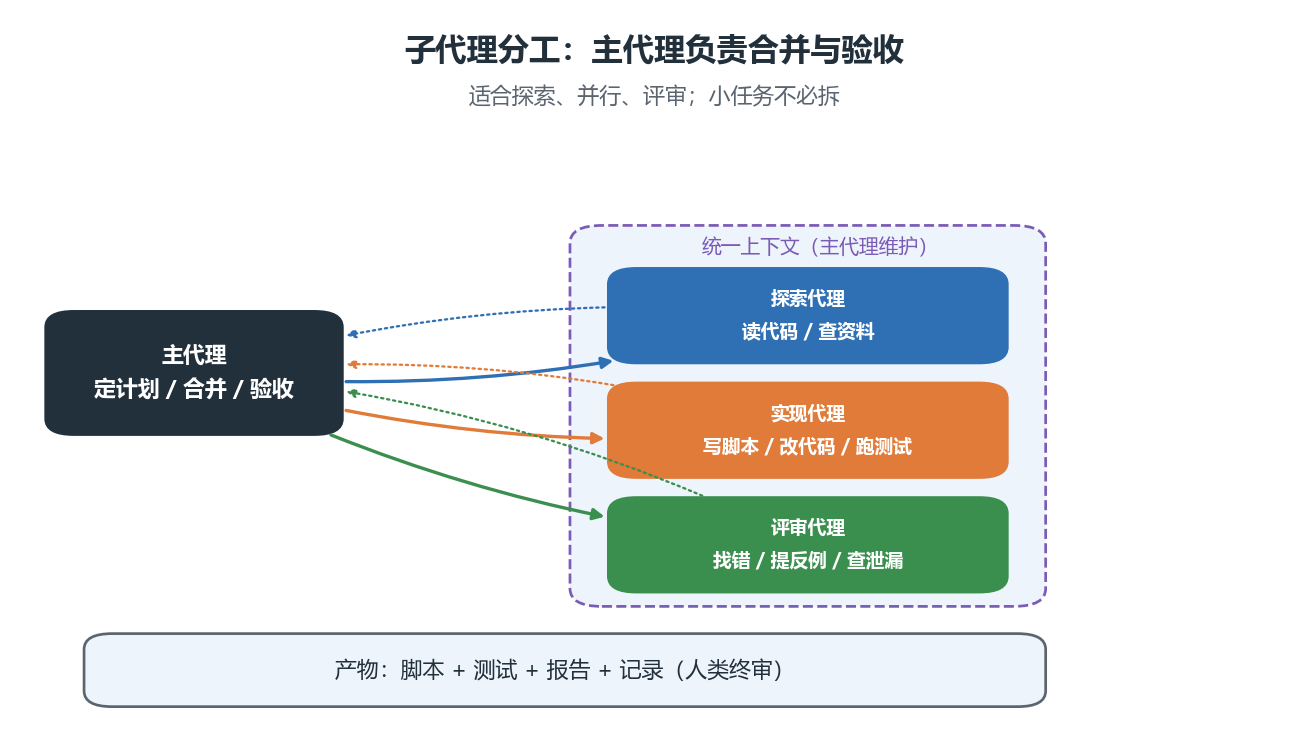
\includegraphics[keepaspectratio,alt={子代理分工}]{figures/11-agent-cases/subagent_split.png}}
\caption{子代理分工}
\end{figure}

{\def\LTcaptype{none} % do not increment counter
\begin{longtable}[]{@{}
  >{\raggedright\arraybackslash}p{(\linewidth - 6\tabcolsep) * \real{0.2500}}
  >{\raggedright\arraybackslash}p{(\linewidth - 6\tabcolsep) * \real{0.2500}}
  >{\raggedright\arraybackslash}p{(\linewidth - 6\tabcolsep) * \real{0.2500}}
  >{\raggedright\arraybackslash}p{(\linewidth - 6\tabcolsep) * \real{0.2500}}@{}}
\toprule\noalign{}
\begin{minipage}[b]{\linewidth}\raggedright
角色
\end{minipage} & \begin{minipage}[b]{\linewidth}\raggedright
输入
\end{minipage} & \begin{minipage}[b]{\linewidth}\raggedright
产出
\end{minipage} & \begin{minipage}[b]{\linewidth}\raggedright
你要做的检查
\end{minipage} \\
\midrule\noalign{}
\endhead
\bottomrule\noalign{}
\endlastfoot
探索代理 & 数据集与题目 & 特征分布、类别平衡、3 条建模建议 &
建议是否与数据事实一致 \\
实现代理 & 任务卡 + AGENTS.md & 脚本、输出文件 & 是否动了不该动的文件 \\
评审代理 & 只给 \texttt{src/} 与 \texttt{output/} & ≥3 条质疑 &
质疑是否被逐条回应 \\
\end{longtable}
}

\subsection{验收标准（可执行，已运行核验）}\label{ux9a8cux6536ux6807ux51c6ux53efux6267ux884cux5df2ux8fd0ux884cux6838ux9a8c-3}

\begin{Shaded}
\begin{Highlighting}[]
\ImportTok{import}\NormalTok{ numpy }\ImportTok{as}\NormalTok{ np}
\ImportTok{from}\NormalTok{ sklearn.datasets }\ImportTok{import}\NormalTok{ load\_wine}
\ImportTok{from}\NormalTok{ sklearn.linear\_model }\ImportTok{import}\NormalTok{ LogisticRegression}
\ImportTok{from}\NormalTok{ sklearn.model\_selection }\ImportTok{import}\NormalTok{ cross\_val\_score}
\ImportTok{from}\NormalTok{ sklearn.pipeline }\ImportTok{import}\NormalTok{ make\_pipeline}
\ImportTok{from}\NormalTok{ sklearn.preprocessing }\ImportTok{import}\NormalTok{ StandardScaler}

\NormalTok{X, y }\OperatorTok{=}\NormalTok{ load\_wine(return\_X\_y}\OperatorTok{=}\VariableTok{True}\NormalTok{)}
\NormalTok{pipe }\OperatorTok{=}\NormalTok{ make\_pipeline(StandardScaler(), LogisticRegression(max\_iter}\OperatorTok{=}\DecValTok{5000}\NormalTok{))}
\NormalTok{scores }\OperatorTok{=}\NormalTok{ cross\_val\_score(pipe, X, y, cv}\OperatorTok{=}\DecValTok{5}\NormalTok{)}

\ControlFlowTok{assert} \BuiltInTok{len}\NormalTok{(pipe.steps) }\OperatorTok{==} \DecValTok{2} \KeywordTok{and}\NormalTok{ pipe.steps[}\DecValTok{0}\NormalTok{][}\DecValTok{0}\NormalTok{] }\OperatorTok{==} \StringTok{"standardscaler"}\NormalTok{, }\StringTok{"标准化必须在 Pipeline 内"}
\ControlFlowTok{assert}\NormalTok{ scores.}\BuiltInTok{min}\NormalTok{() }\OperatorTok{\textgreater{}} \FloatTok{0.9}\NormalTok{, }\StringTok{"5 折最低分不应低于 0.90"}

\BuiltInTok{print}\NormalTok{(}\StringTok{"5 折准确率:"}\NormalTok{, np.}\BuiltInTok{round}\NormalTok{(scores, }\DecValTok{4}\NormalTok{))}
\BuiltInTok{print}\NormalTok{(}\StringTok{"均值:"}\NormalTok{, }\BuiltInTok{round}\NormalTok{(}\BuiltInTok{float}\NormalTok{(scores.mean()), }\DecValTok{4}\NormalTok{))}
\BuiltInTok{print}\NormalTok{(}\StringTok{"结构检查通过：标准化在 Pipeline 内，无全局预处理泄漏"}\NormalTok{)}
\end{Highlighting}
\end{Shaded}

\begin{Shaded}
\begin{Highlighting}[]
\NormalTok{5 折准确率: [0.9722 0.9722 1.     0.9714 1.    ]}
\NormalTok{均值: 0.9832}
\NormalTok{结构检查通过：标准化在 Pipeline 内，无全局预处理泄漏}
\end{Highlighting}
\end{Shaded}

\begin{quote}
注意：\texttt{scores.min()\ \textgreater{}\ 0.9}
这样的阈值来自\textbf{你对任务的要求}，不是模型自带的结论；如果你换数据集，阈值必须重设------这正是''验收标准由人定义''。
\end{quote}

\subsection{人工复核点}\label{ux4ebaux5de5ux590dux6838ux70b9-2}

\begin{enumerate}
\def\labelenumi{\arabic{enumi}.}
\tightlist
\item
  \textbf{数据泄漏}：标准化、特征选择、降维是否都在 Pipeline
  内（在划分之前做 = 泄漏）；
\item
  \textbf{指标口径}：交叉验证与测试集指标不能混用一句话描述；
\item
  \textbf{报告一致性}：报告里的每个数字都能在 \texttt{output/}
  里找到出处；
\item
  \textbf{评审闭环}：评审意见不能只有''已修复''，要写清怎么改、改后指标变化；
\item
  \textbf{AI 使用声明}：写明哪些环节用了 Agent、你做了哪些修改（模板见
  08 节）。
\end{enumerate}

\subsection{离线替代路径}\label{ux79bbux7ebfux66ffux4ee3ux8defux5f84-2}

无网络时：仍可完成本案例（sklearn 数据自带、脚本本地跑）；把''Agent
产出''换成 \texttt{lab/sample\_agent\_output/}
的参考实现，你扮演评审代理，练习写 \texttt{review.md} 与逐条回应。

\subsection{常见坑}\label{ux5e38ux89c1ux5751-3}

{\def\LTcaptype{none} % do not increment counter
\begin{longtable}[]{@{}
  >{\raggedright\arraybackslash}p{(\linewidth - 4\tabcolsep) * \real{0.3333}}
  >{\raggedright\arraybackslash}p{(\linewidth - 4\tabcolsep) * \real{0.3333}}
  >{\raggedright\arraybackslash}p{(\linewidth - 4\tabcolsep) * \real{0.3333}}@{}}
\toprule\noalign{}
\begin{minipage}[b]{\linewidth}\raggedright
坑
\end{minipage} & \begin{minipage}[b]{\linewidth}\raggedright
后果
\end{minipage} & \begin{minipage}[b]{\linewidth}\raggedright
避免方式
\end{minipage} \\
\midrule\noalign{}
\endhead
\bottomrule\noalign{}
\endlastfoot
让 Agent 一把梭完成整个项目 & 过程不可解释，出错难定位 &
先计划模式，再分阶段执行 \\
报告由 Agent 直接生成、数字对不上 & 数据与结论脱节 &
报告中的数字必须来自 \texttt{output/} \\
评审代理与实现代理''同一视角'' & 挑不出真问题 &
评审只给代码与输出，不给你的解释 \\
忘记 LaTeX 编译验证 & 提交的 tex 编不过 & 验收标准里加''编译成功并附
PDF'' \\
\end{longtable}
}

\subsection{拓展}\label{ux62d3ux5c55-14}

\begin{enumerate}
\def\labelenumi{\arabic{enumi}.}
\tightlist
\item
  换成题目 B（交通网络），比较两种任务下 Agent 的表现差异；
\item
  引入''红队''环节：让评审代理专门构造能骗过指标的测试样例（例如类别不平衡）；
\item
  把整个项目接进 git：每个阶段一次提交，最后用 \texttt{git\ log}
  复盘''哪些改动来自 Agent、哪些来自你''。
\end{enumerate}

\subsection{练习与延伸阅读}\label{ux7ec3ux4e60ux4e0eux5ef6ux4f38ux9605ux8bfb-6}

\begin{itemize}
\tightlist
\item
  练习：exercises/assignment.md 第 11--12 题（项目复盘 + AI 使用声明）；
\item
  上机：lab/lab.ipynb Part C（综合任务）；
\item
  延伸：第 8 章综合案例、期末大作业项目 1 / 2。
\end{itemize}

\newpage
